\graphicspath{{images/}}

\section{\thesection~Results}
\label{sec:results}


% \subsection{\thesubsection~Guessing}
% \end{multicols}
% \graphicspath{{images/guessing/}}
% \begin{Figure}
%   \centering
%   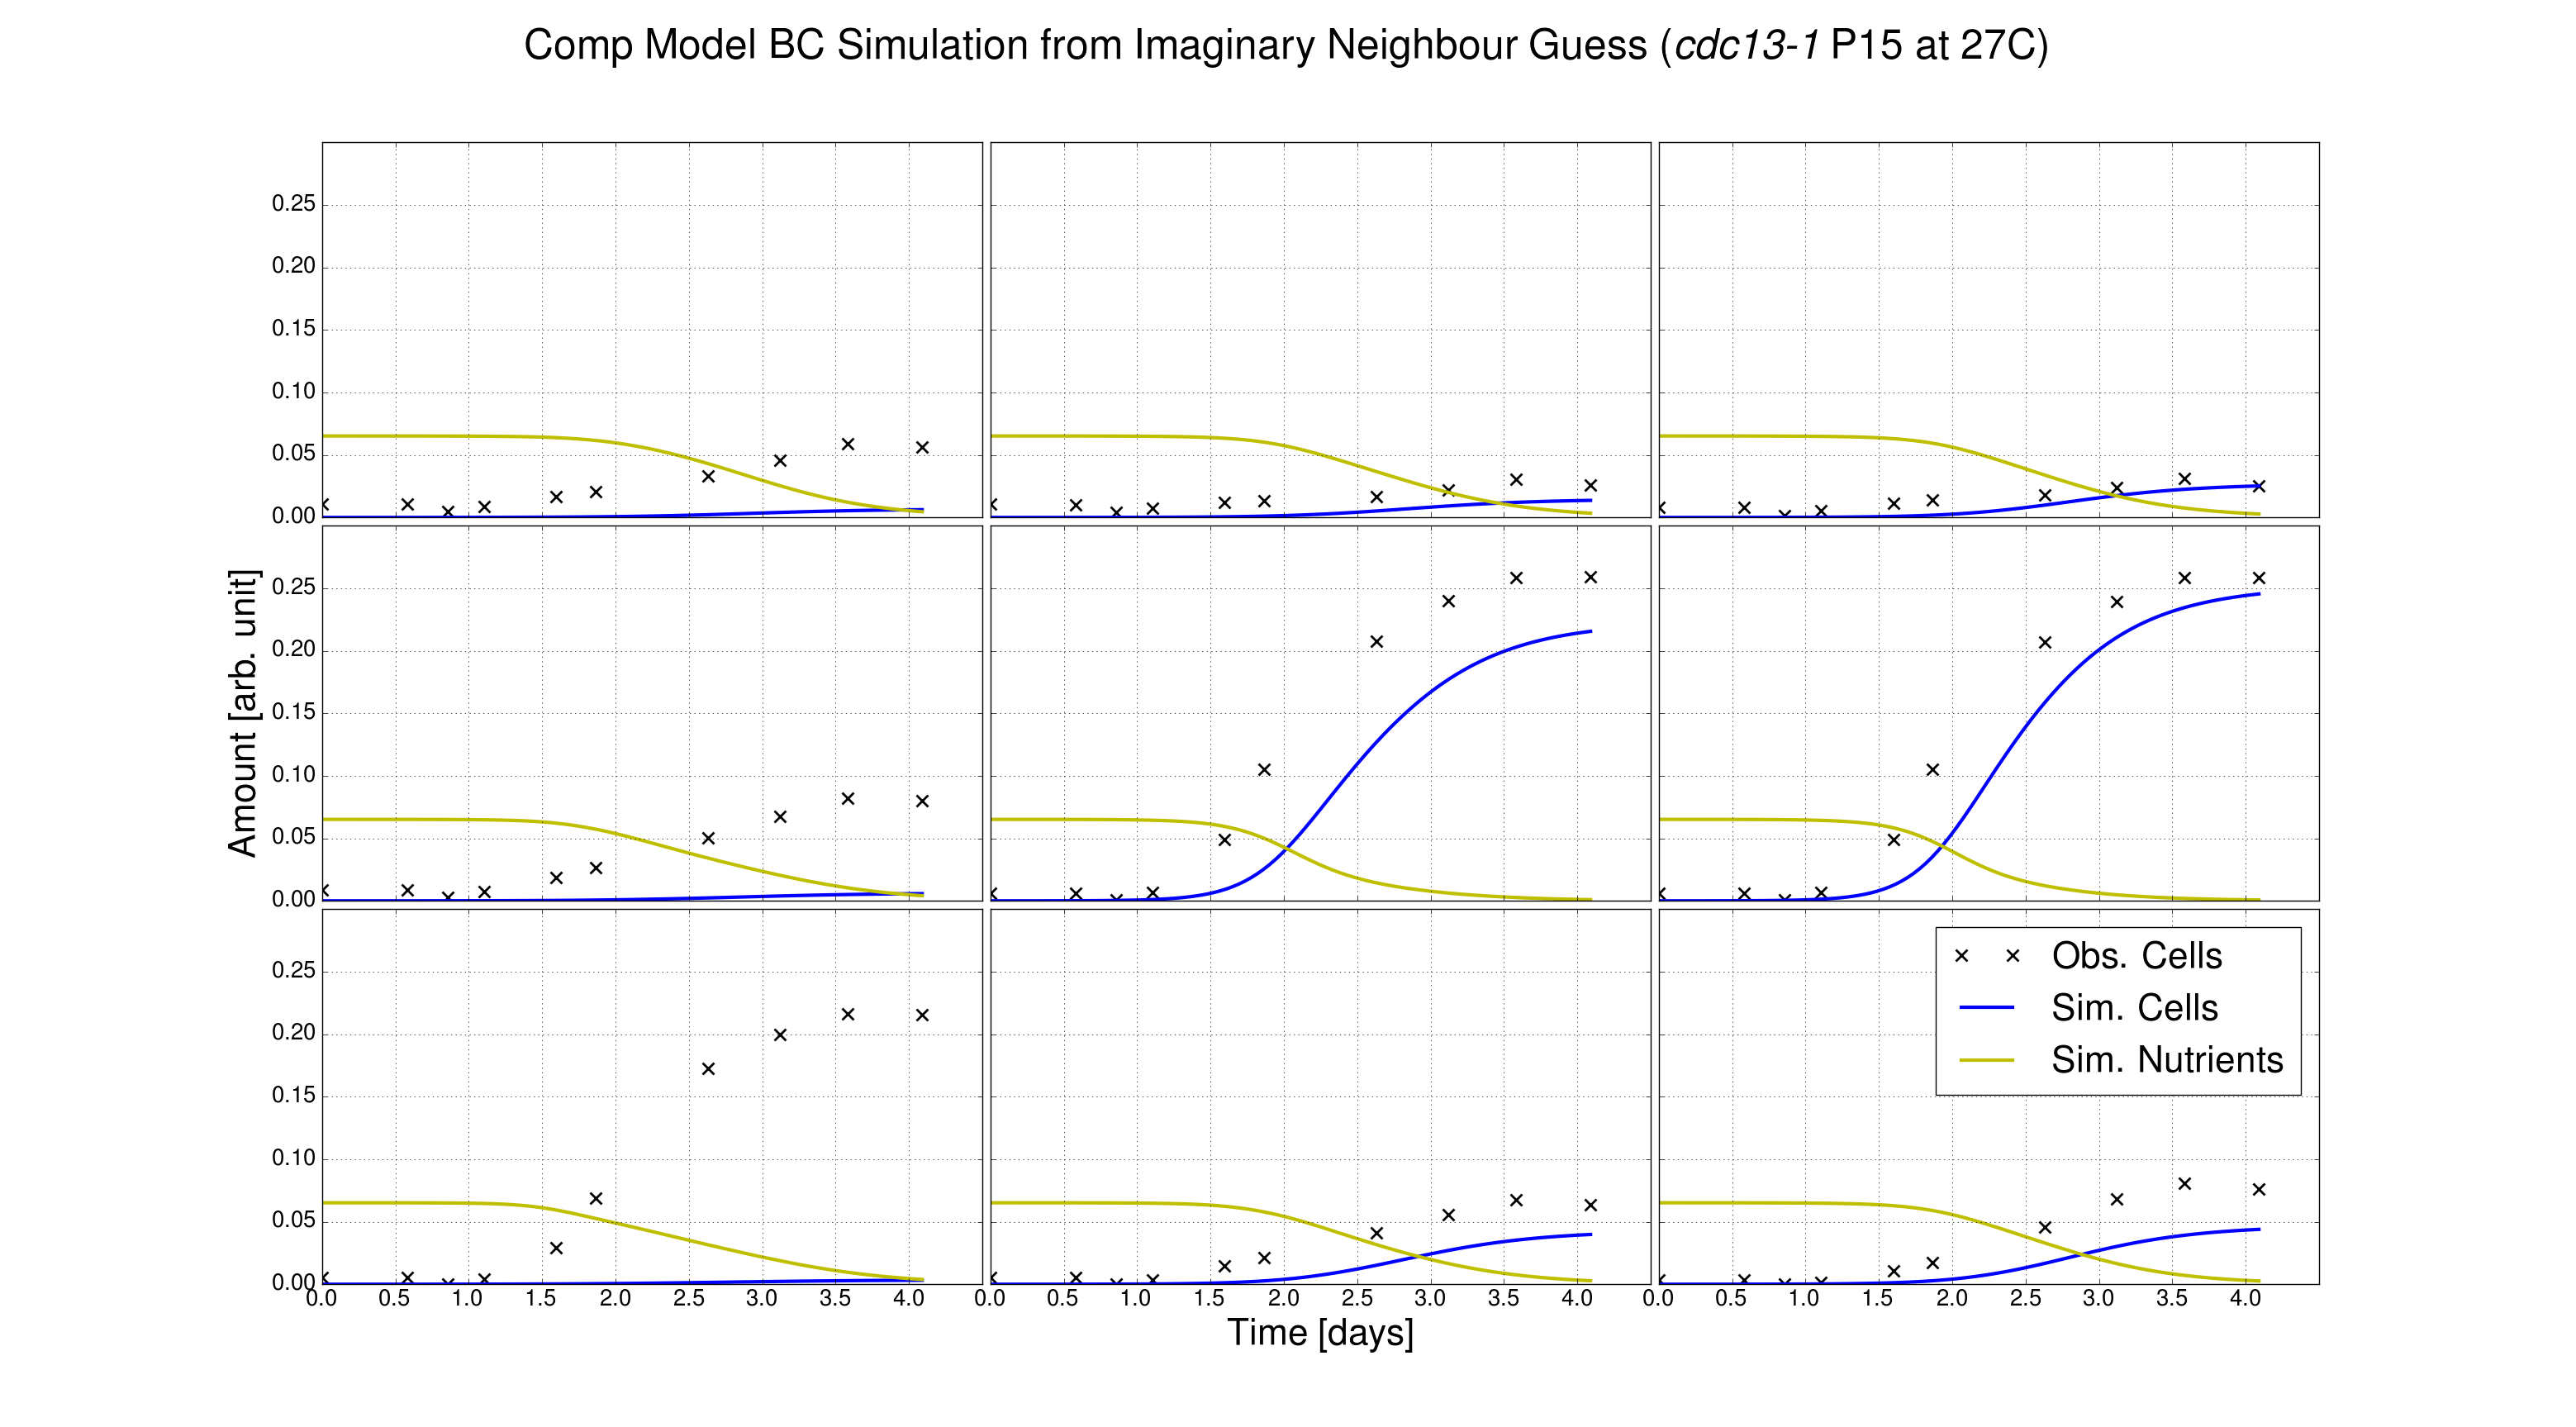
\includegraphics[width=\linewidth]{final/P15_R5_C18_guess_sim}
%   \captionof{figure}{\textbf{Competition model simulation using
%       parameters from imaginary neighbour guessing.} Shows a 3x3 zone
%     with top-left coordinate (5, 18) from P15 with background
%     \textit{cdc13-1} at 27\(^{\circ}C\).}
%   \label{fig:imag_neigh_guess_sim}
% \end{Figure}
% \begin{multicols}{2}

% Scripts were run with combinations of the following values.
% cellratios = np.logspace(-3, -5, num=5)
% fittype = ["imagneigh", "logeq"]
% zerokn = [True, False]

% Each script looped through the following array of b values which were
% supplied to the initial guesser and used at the plate level.

% for b-guess in [35, 40, 45, 50, 55, 60, 65, 70, 75, 80, 95, 100, 150]:

\subsection{\thesubsection~Model comparison using P15}

I ran multiple fits of the competition model to P15 (see
Section~\ref{sec:P15_description}). Each fit used the imaginary
neighbour model to make initial parameter guesses (see
Section~\ref{sec:guessing_b}. The imaginary neighbour model itself
requires initial parameters and fits looped over combinations of
values for initial cell density \(C(0)\) and growth constant \(b\). I
used five initial values of \(C(0)\) ranging from
\(N(0)\times\)10\(^{-5}\) to \(N(0)\times\)10\(^{-3}\) in logspace
(\(N(0)\) is approximately equal to final cells) and a range of 14
different values for \(b\) as described in
Section~\ref{sec:guessing_b}. This made a total of 70 fits. I show
estimated competition model parameters for the two best fits in
Table~\ref{tab:P15_best_fit_params}. Estimated initial nutrient
amounts agree fairly well between but there is disagreement in
estimates of \(C(0)\) and (nutrient diffusion constant) \(k\). It
appears that the gradient method is not finding a global
minimum. However, \(b_{i}\) estimates were correlated with Spearman's
rank correlation coefficient, \(\rho_{S} = 0.989\), and had average
mean absolute deviation, \(MAD = 1.56\). The mean of \(b_{i}\)
estimates for the best fit was 44.4.

\begin{center}
  \captionof{table}{\textbf{Estimated parameter values for the best
      two competition model fits to P15.} Spearman's rank correlation
    coefficient between \(b_{i}\) estimates, \(\rho_{S}\) =
    0.989. Mean absolute deviation between \(b_{i}\) estimates, MAD =
    1.56. The total objective function value for internal cultures is
    shown in the last column.}
  \begin{tabular}{l l l l l l}
    \hline
    Fit     & \(C(0)\)                    & \(N_{I}(0)\) & \(N_{E}(0)\) & \(k\) & Obj.\\
    \hline
    1st     & 9.1\(\times\)10\(^{-5}\)    & 0.064      & 0.090       & 6.7  & 0.194 \\
    2nd     & 13.9\(\times\)10\(^{-5}\)   & 0.062      & 0.097       & 8.3  & 0.196 \\
    \hline
  \end{tabular}
  \label{tab:P15_best_fit_params}
\end{center}


For all comparisons between the top four fits \(\rho_{S}\) ranges from
0.922 to 0.995 and \(b\) MAD ranges from 1.56 to 6.90. I discarded the
5th best fit, which has less agreement, because, unlike the other
fits, it estimated \(N_{I}(0)\) > \(N_{E}(0)\). When comparing to the
top four fits, \(\rho_{S}\) was above 0.930 but \(b\) values were more
affected with a maximum MAD of 13.29. Despite not finding a global
minimum, the best competition model estimates agree well enough with
each other to make meaningful comparison with logistic model
estimates.


%%%%

The best fit of the competition model to P15 is shown in
Figure~\ref{fig:comp_fit_plate}. The estimated cell amounts (blue)
match the data well across the entire plate. Fits of the competition
model (solid), imaginary neighbour guess (dashed), and logistic model
(red) are plotted for a 3x3 zone in Figure~\ref{fig:P15_zone_fit}.
% could have a table with initial guess
The logistic model was fit using the QFA R package \citep{qfa2016}.
The fit of the initial guess is typical for the plate. Some culture,
such as the bottom-left, are not well fit. However, Spearman's
\(\rho_{s}\) for the imaginary neighbour guess and competition model
\(b_{i}\) estimates is (fill ) and the guess leads to a good fit when
used to initialise parameters of the competition model. Over the
plate, the logistic model and competition model perform similarly
(Table\ref{tab:P15_obj_fun}) .

the zone contains more fast growing cultures than is average for the
plate.

% For the I discard Observations of edge culture are noisy due to reflections from plate
% walls and estimates are usually discarded.





\graphicspath{{images/p15_fits/}}
\begin{Figure}
  \centering
  \includegraphics[width=\linewidth]{final/zone_r5_c18_with_obj_fun}
  \captionof{figure}{\textbf{Comparison of competition and logistic
      model fits to a zone of P15}. The logistic model was fit with
    the QFA R package and uses almost three times as many
    parameters. The initial guess for the competition model (dashes)
    was made from fits of the imaginary neighbour model to individual
    cultures. The zone has top-left coordinates (5, 18) and is boxed
    in red in Figure~\ref{fig:comp_fit_plate}. Objective function
    values for each culture (Obj.) were scaled by \(10^{4}\).}
  \label{fig:P15_zone_fit}
\end{Figure}



\begin{center}
  \captionof{table}{\textbf{Objective function values for fits to
      P15.} ``Internal'' is the total objective function value for
    cultures not at an edge. ``All'' is the total objective function
    value for all cultures on the plate.}
  \begin{tabular}{l l l}
    \hline
    Cultures     & Competition & Logistic \\
    \hline
    Internal     & 0.194    & 0.155\\
    All          & 0.465    & 0.345\\
    \hline
  \end{tabular}
  \label{tab:P15_obj_fun}
\end{center}


\graphicspath{{images/p15_correlations/}}
\begin{Figure}
  \centering
  \includegraphics[width=\linewidth]{final/r_correlations_median_spearmans_trimmed}
  \captionof{figure}{\textbf{Correlation between logistic and
      competition model r estimates for P15}. Correlations are plotted
    between r estimates for each culture (black) and between medians
    of r estimates for each deletion (red). There were six repeats in
    random locations per deletion (except for the neutral deletion
    \textit{his3\(\Delta\)} which had 14). Logistic fits used the QFA
    R package. Spearman's rank correlation coefficient, \(\rho_{s}\),
    is shown for each distribution. The line y = x is also plotted.}
  \label{fig:P15_correlations}
\end{Figure}


% Complicated correlation coefficient table
% \columnbreak
% \begin{center}
%   \captionof{table}{\textbf{Correlation coefficients between logistic
%       and competition model estimates of parameters for P15.} Pearson
%     correlation coefficient \(\rho\) and Spearman rank correlation
%     coefficient \(r_{s}\) are shown. Correlation coefficients compare
%     between logistic and competition model estimates for both \(r\)
%     and \(MDR\). Correlations are shown between estimates for each
%     culture and between median and mean estimates for each deletion.}
% \begin{tabular}{ |c|c|c|c|c| } \cline{2-5}
% \multicolumn{1}{c|}{} & \multicolumn{2}{c|}{\(r\)} & \multicolumn{2}{c|}{\(MDR\)}\\ \hline
% \multicolumn{1}{|c|}{Estimates} & \(\rho\) & \(r_{s}\) & \(\rho\) & \(r_{s}\)\\ \hline
% Culture & 0.712 & 0.731 & 0.752 & 0.754\\
% Median & 0.708 & 0.497 & 0.791 & 0.635\\
% Mean   & 0.763 & 0.594 & 0.885 & 0.732\\ \hline
% \end{tabular}
% \end{center}

% Just a fit of a zone
% \end{multicols}
% \graphicspath{{images/comp_fit/}}
% \begin{Figure}
%   \centering
%   \includegraphics[width=\linewidth]{final/P15_guess_and_fit_r5_c18}
%   \captionof{figure}{\textbf{A zone of a fit of the competition model
%       to P15 and initial guess}. The guess was made using the
%     imaginary neighbour model fit to individual cultures. Top-left
%     coordinates from Figure~\ref{fig:comp_fit_plate} (5, 18).}
%   \label{fig:comp_fit_zone_old}
% \end{Figure}
% \begin{multicols}{2}

  Some text Some text Some text Some text Some text Some text Some
  text Some text Some text Some text Some text Some text Some text
  Some text Some text Some text Some text Some text Some text Some
  text Some text Some text Some text Some text Some text Some text
  Some text Some text Some text Some text Some text Some text Some
  text Some text Some text Some text Some text Some text Some text
  Some text Some text Some text Some text Some text Some text Some
  text Some text Some text Some text Some text Some text Some text
  Some text Some text Some text Some text Some text Some text Some
  text Some text Some text Some text Some text Some text Some text
  Some text Some text Some text Some text Some text Some text Some
  text Some text Some text Some text Some text Some text Some text
  Some text Some text Some text Some text Some text Some text Some
  text Some text Some text Some text Some text Some text Some text
  Some text Some text Some text Some text Some text Some text Some
  text Some text Some text Some text Some text Some text Some text
  Some text Some text Some text Some text.


% Make landscape and take a whole page.
\end{multicols}
\begin{landscape}
\graphicspath{{images/comp_fit/}}
\begin{Figure}
  \centering
  \includegraphics[width=\linewidth]{full_plate/final/P15_12x20}
  \captionof{figure}{\textbf{Fit of the competition model to P15.}
    Data is for a 16x24 format plate (P15) with a background mutation
    \textit{cdc13-1} incubated at 27\(^{\circ}C\). The plate contains
    6 repeats of 50 genetic strains randomly arranged across the
    internal cultures. Repeats of a single strain are used for all
    edge cultures (removed in the plot). Model output for state
    variable, cell population size (blue curve), is fit to observed
    data (black crosses). Model predictions for unobserved variable
    (nutrient amount) are also plotted (yellow).}
  \label{fig:comp_fit_plate}
\end{Figure}
\end{landscape}
\begin{multicols}{2}


\subsection{\thesubsection~Evaluating the treatment of boundaries}

\graphicspath{{images/corners/}}
\begin{Figure}
  \centering
  \includegraphics[width=\linewidth]{final/top_left_new_aspect}
  \captionof{figure}{\textbf{Treatment of boundary conditions in fits
      of the competition model.} The top left corner of a 16x24 QFA
    plate fitted with two versions of the competition model, the first
    has a single initial nutrient amount for all cultures, the second
    has a separate initial nutrient amount for edge cultures.}
  \label{fig:P15_corner}
\end{Figure}

% Alternate version with legend in separate image
% \graphicspath{{images/corners/}}
% \begin{Figure}
%   \centering
%   \includegraphics[width=\linewidth]{final/top_left_new_aspect_sans_legend}
%   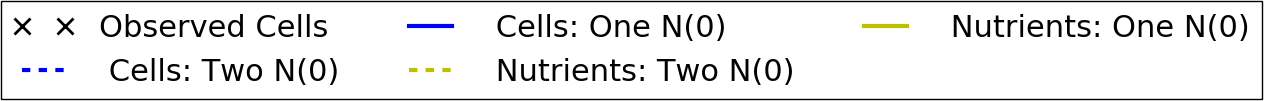
\includegraphics[width=\linewidth]{final/legend}
%   \captionof{figure}{\textbf{Treatment of boundary conditions in fits
%       of the competition model.} The top left corner of a 16x24 QFA
%     plate fitted with two versions of the competition model, the first
%     has a single initial nutrient amount for all cultures, the second
%     has a separate initial nutrient amount for edge cultures.}
%   \label{fig:P15_corner_2}
% \end{Figure}


\begin{center}
  \captionof{table}{\textbf{Average objective function value for one a
      two \(\bm{N(0)}\) parameter competition models.} Values are for
    the same fits as in Figure~\ref{fig:P15_corner} and have been
    scaled by \(10^{4}\). Averages are for cultures belonging to the
    areas indicated by the column ``Cultures''. ``Next to edge''
    refers to cultures one in from the edge. ``Internal'' refers to
    all cultures but the edge.}
  \begin{tabular}{l l l}
    \hline
    Cultures     & One \(N(0)\)  & Two \(N(0)\) \\
    \hline
    Edge         & 35.9    & 36.5\\
    Next to edge & 9.54    & 7.98\\
    Internal     & 6.67    & 6.30\\
    All          & 12.4    & 12.2\\
    \hline
  \end{tabular}
  \label{tab:corner}
\end{center}

Table~\ref{tab:corner}

  Some text Some text Some text Some text Some text Some text Some
  text Some text Some text Some text Some text Some text Some text
  Some text Some text Some text Some text Some text Some text Some
  text Some text Some text Some text Some text Some text Some text
  Some text Some text Some text Some text Some text Some text Some
  text Some text Some text Some text Some text Some text Some text
  Some text Some text Some text Some text Some text Some text Some
  text Some text Some text Some text Some text Some text Some text
  Some text Some text Some text Some text Some text Some text Some
  text Some text Some text Some text Some text Some text Some text
  Some text Some text Some text Some text Some text Some text Some
  text Some text Some text Some text Some text Some text Some text
  Some text Some text Some text Some text Some text Some text Some
  text Some text Some text Some text Some text Some text Some text
  Some text Some text Some text Some text Some text Some text Some
  text Some text Some text Some text Some text Some text Some text
  Some text Some text Some text Some text.

\subsection{\thesubsection~Agreement of b rankings}

  Some text Some text Some text Some text Some text Some text Some
  text Some text Some text Some text Some text Some text Some text
  Some text Some text Some text Some text Some text Some text Some
  text Some text Some text Some text Some text Some text Some text
  Some text Some text Some text Some text Some text Some text Some
  text Some text Some text Some text Some text Some text Some text
  Some text Some text Some text Some text Some text Some text Some
  text Some text Some text Some text Some text Some text Some text
  Some text Some text Some text Some text Some text Some text Some
  text Some text Some text Some text Some text Some text Some text
  Some text Some text Some text Some text Some text Some text Some
  text Some text Some text Some text Some text Some text Some text
  Some text Some text Some text Some text Some text Some text Some
  text Some text Some text Some text Some text Some text Some text
  Some text Some text Some text Some text Some text Some text Some
  text Some text Some text Some text Some text Some text Some text
  Some text Some text Some text Some text.
% \graphicspath{{images/rank/}}
% \begin{Figure}
%   \centering
%   \includegraphics[width=\linewidth]{top_two_comp_p15_correlations_trimmed}
%   \captionof{figure}{\textbf{Comparison of \(\bm{b}\) ranking for the
%       best five competition model fits to P15.} Ranking is calculated
%     from the mean \(b\) estimate from the six repeats or each strain.}
%   \label{fig:comp_b_ranking}
% \end{Figure}

\subsection{\thesubsection~Comparison of fitness ranking}

\graphicspath{{images/rank/}}
\begin{Figure}
  \centering
  \includegraphics[width=\linewidth]{final/median_ranks_comp_b_log_r_MDR}
  \captionof{figure}{\textbf{Comparison of \(\bm{r}\) ranking for fits
      of the competition and logistic model to P15.} Rankings are
    determined from median parameter estimates for repeats of each
    deletion. Competition model \(r\) was converted from \(b\),
    \(N_0\), and \(C_0\) from the best competition model
    estimate. Logistic \(r\) was taken from fits using the QFA R
    package which makes heuristic checks for slow growing cultures.
    For competition \(b\) and logistic \(r\), \(\rho_{S} = 0.497\);
    for competition \(b\) and logistic \(MDR\), \(\rho_{S} = 0.635\).}
  \label{fig:comp_vs_log_ranking}
\end{Figure}


% \graphicspath{{images/rank/}}
% \begin{Figure}
%   \centering
%   \includegraphics[width=\linewidth]{final/comp_b_log_r_trimmed}
%   \captionof{figure}{\textbf{Comparison of \(\bm{r}\) ranking for fits
%       of the competition and logistic model to P15.} Fitnesses of
%     genetic strains are ranked most to least fit from top to
%     bottom. Competition model \(r\) was converted from \(b\), \(N_0\),
%     and \(C_0\) from the best competition model estimate. Logistic
%     \(r\) and \(MDR\) were taken from logistic model fits using the
%     QFA R package which makes heuristic checks for slow growing
%     cultures.}
%   \label{fig:comp_vs_log_ranking2}
% \end{Figure}

\subsection{\thesubsection~Comparison of Variation in Fitness Estimates}

Use repeats on plate 15 (6 per deletion) more (14) for HIS3 to
calculate coefficient of variation (COV) of estimated r or MDR.

\end{multicols}
\graphicspath{{images/COV/}}
\begin{Figure}
  \centering
  \includegraphics[width=\linewidth]{final/comp_b_log_r_median_rank_his3_bold}
  \captionof{figure}{\textbf{Coefficient of variation (COV) for growth
      estimates from P15.} COVs are shown for competition model \(b\)
    and logistic model \(r\) for repeats of each deletion. COVs of
    competition model \(b\) and \(r\) are equivalent (see
    Section~\ref{sec:parameter_conversion}). Deletions are ordered
    left to right along the horizontal axis by highest to lowest
    competition model \(b\) ranking. Logistic fits used the QFA R
    package.}
  \label{fig:comp_b_log_r}
\end{Figure}
\begin{multicols}{2}

\subsection{\thesubsection~Cross-plate validation}

\end{multicols}
\graphicspath{{images/stripes/}}
\begin{Figure}
  \centering
  \includegraphics[width=\linewidth]{final/validation_r9_c10_no_nutrients}
  \captionof{figure}{\textbf{Calibration and validation of the
      competition model.} I fit the competition model to the 16x24
    format ``Stripes'' and ``Filled'' plates in
    Figure~\ref{fig:stripes_images}. The plot shows cell measurements
    and estimates for both plates for a 3x3 section with top left
    coordinates (R9, C10). I took the parameters estimates for the
    ``Filled'' plate (calibration) and set growth constant, b, to zero
    for cultures in the empty columns of the ``Stripes'' plate. I then
    simulated using these parameters to produce the dashed blue curve
    (validation). If the model corrects for differences in growth
    between these experimental designs perfectly, the dashed blue
    curves should resemble the ``Stripes'' data (blue crosses) in
    columns one and three. The logistic model would predict no change
    in growth between plates.}
  \label{fig:stripes_validation}
\end{Figure}
\begin{multicols}{2}


% \graphicspath{{images/stripes/}}
% \begin{Figure}
%   \centering
%   \includegraphics[width=\linewidth]{final/r_correlations_between_plates_A}
%   \includegraphics[width=\linewidth]{final/r_correlations_between_models_B_colours_2}
%   \captionof{figure}{\textbf{Correlation of r estimates for
%       ``Stripes'' and ``Filled'' plates.}~A) Correlation of r
%     estimates between plates for logistic and competition
%     models. B) Correlation of r estimates between logistic and
%     competition models for both plates.  I fit the competition model
%     and independent model to the ``Stripes'' and ``Filled'' plates in
%     Figure~\ref{fig:stripes_images}. I converted competition model b
%     to logistic model r. I only used data for cultures that were
%     common between the two plates common and removed edge
%     cultures. Pearson correlation coefficients, \(\rho\), are shown
%     in the legends. The line \(y=x\) is also plotted.}
%   \label{fig:r_correlations_v2}
% \end{Figure}


\graphicspath{{images/stripes/correlations/}}
\begin{Figure}
  \centering
  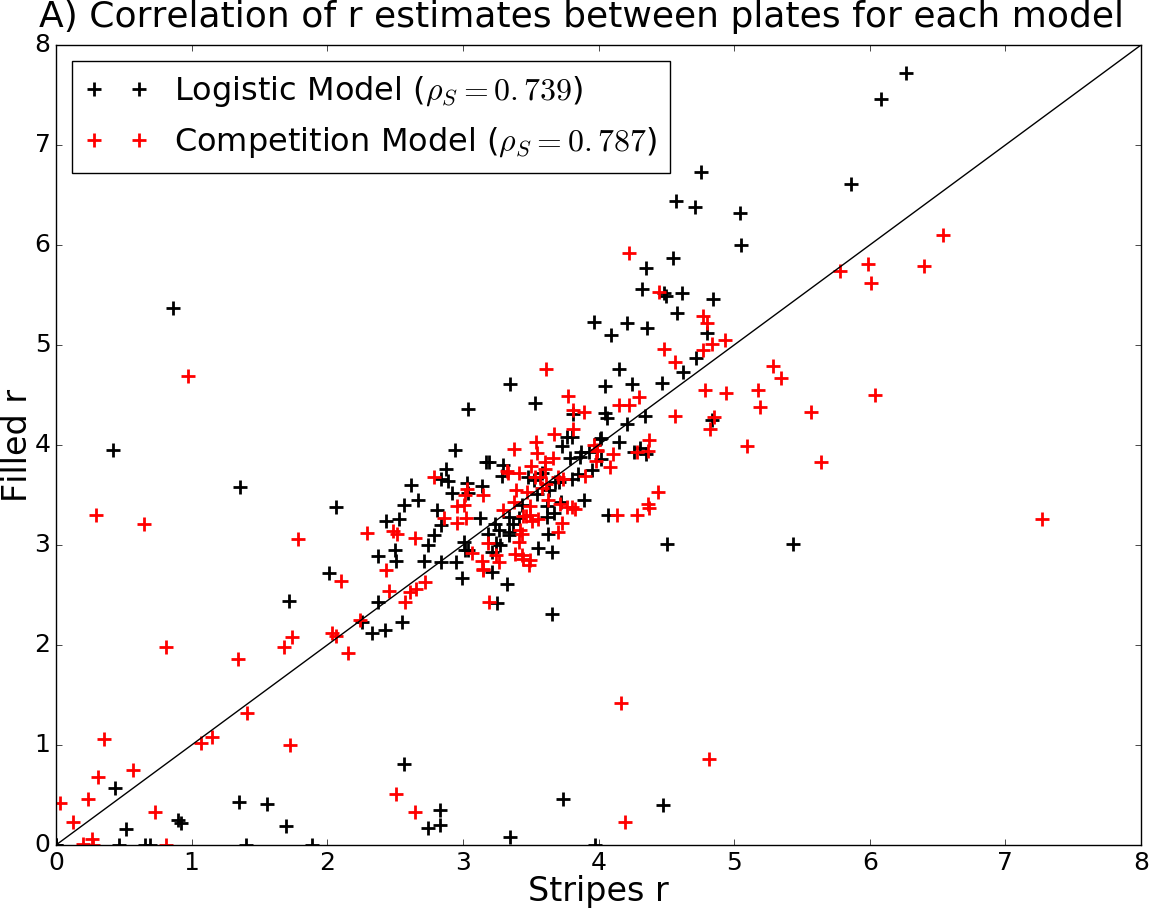
\includegraphics[width=\linewidth]{final/r_correlations_between_plates}
  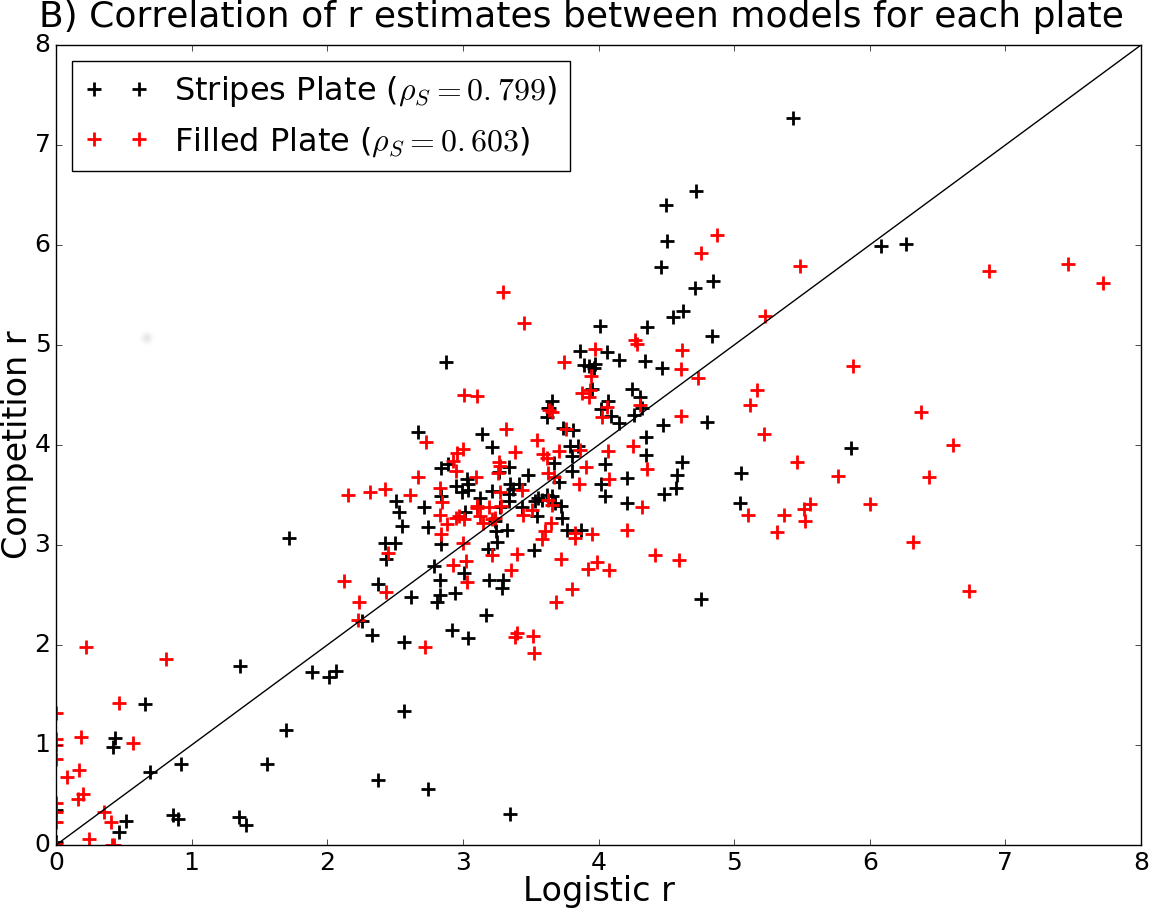
\includegraphics[width=\linewidth]{final/r_correlations_between_models}
  \captionof{figure}{\textbf{Correlation of r estimates for
      ``Stripes'' and ``Filled'' plates.}~I fit the competition model
    and independent model to the ``Stripes'' and ``Filled'' plates in
    Figure~\ref{fig:stripes_images}. I converted competition model b
    to logistic model r. I only used data for cultures that were
    common between the two plates common and removed edge
    cultures. Pearson correlation coefficients, \(\rho\), are shown in
    the legends. The line \(y=x\) is also plotted.}
  \label{fig:r_correlations}
\end{Figure}


\subsection{\thesubsection~Towards a genetic algorithm}

% %\end{multicols}
% \graphicspath{{images/genetic_algorithm/}}
% \begin{Figure}
%   \centering
%   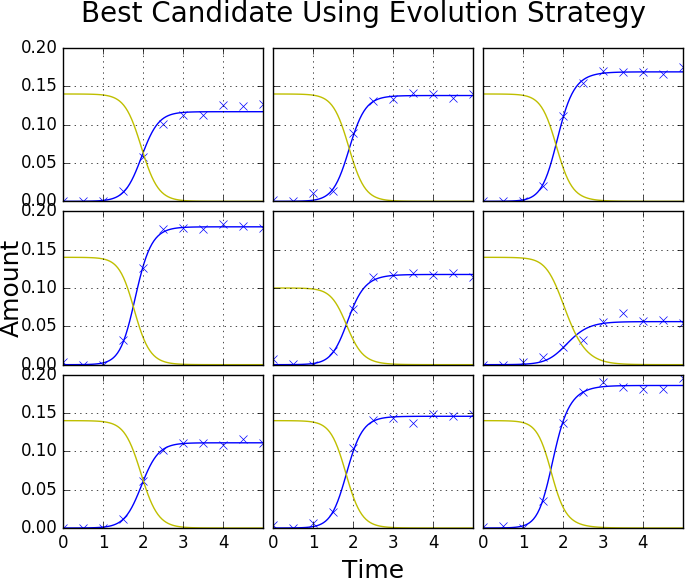
\includegraphics[width=\linewidth]{final/ga_fit_to_sim_true_plate_lvl_trimmed}
%   \captionof{figure}{Genetic algorithm fit to a 3x3 simulation. MIGHT
%     TAKE A LITTLE BIT OF WORK TO REPRODUCE AND COULD USE PARAMETERS
%     FROM THE BEST P15 FIT RATHER THAN JUST PICKING/RANDOMIZING. NEED
%     TO CHECK THAT PLATE LEVEL PARAMETERS WERE ALSO EVOLVED.}
%   \label{fig:3x3_genetic_algorithm_comp_fit_fixed_plate_level}
% \end{Figure}
% %\begin{multicols}{2}


%\end{multicols}
\graphicspath{{images/genetic_algorithm/}}
\begin{Figure}
  \centering
  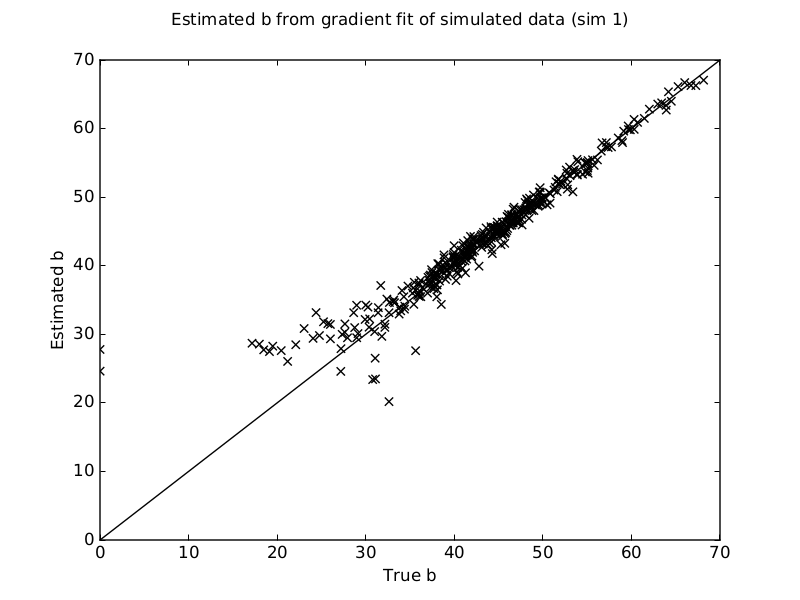
\includegraphics[width=\linewidth]{final/est_b_vs_true_b_imag_neigh_guess_sim_1_trimmed}
  \captionof{figure}{Recovery of true b values from a gradient method
    with fixed plate level parameters. I simulated timecourses from
    the best five competition model fits to p15, fixed the true plate
    level parameters, and used a gradient method to recover b. This
    plot shows the worst case from the five sets of values.}
  \label{fig:comp_fit_fixed_plate_level}
\end{Figure}
%\begin{multicols}{2}

%%% Local Variables:
%%% mode: latex
%%% TeX-master: "report"
%%% End:
